\documentclass{standalone}
\usepackage{tikz}
\usetikzlibrary{patterns, positioning}

\begin{document}
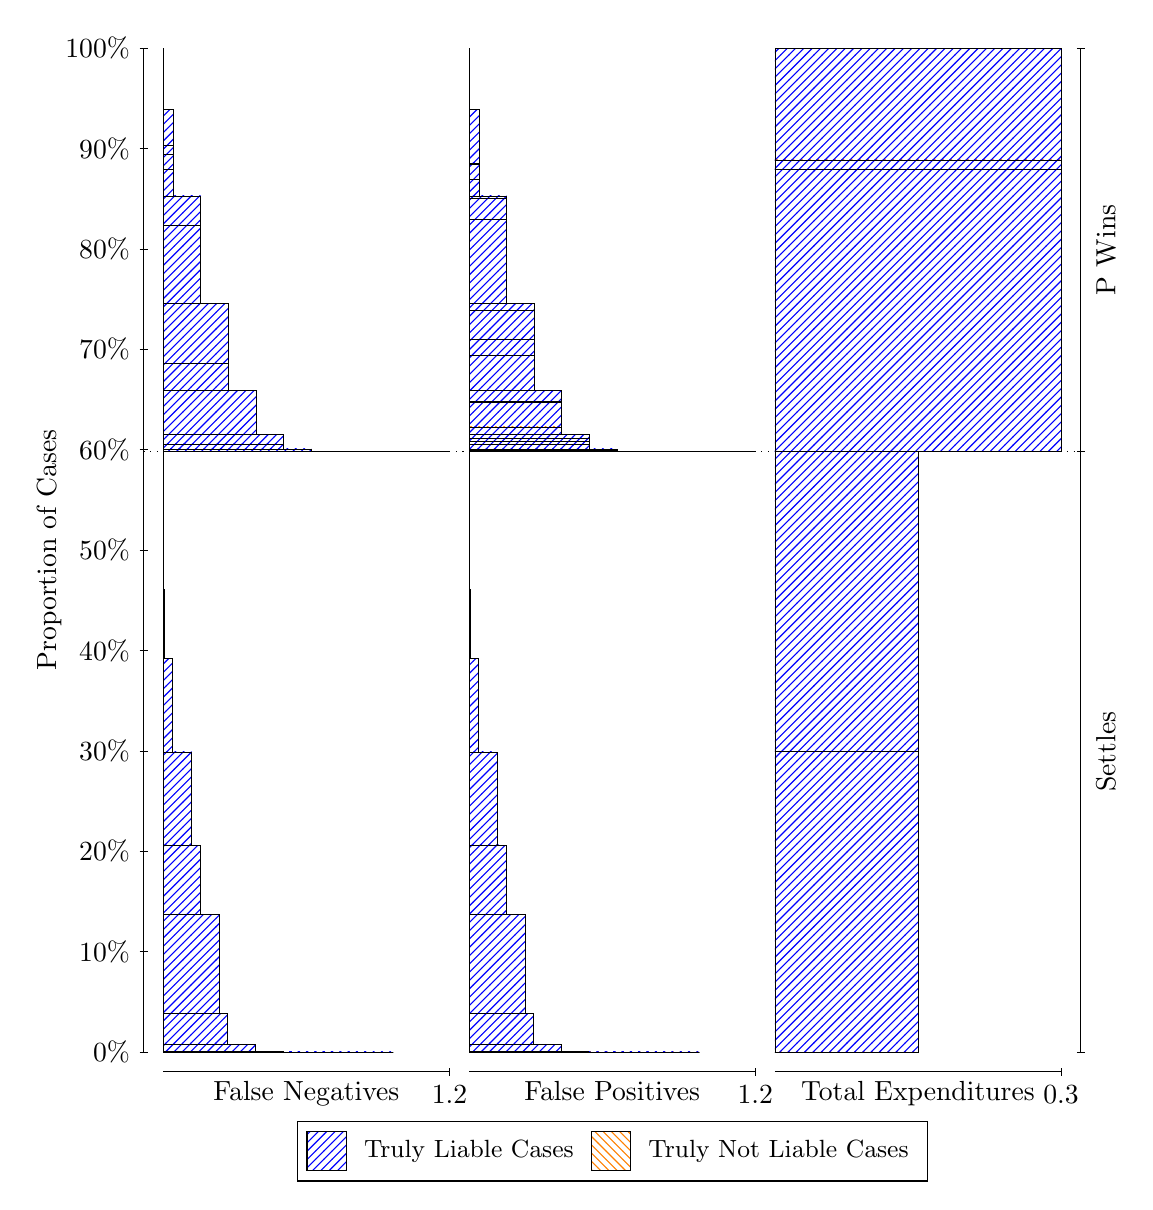
\begin{tikzpicture}
\draw[black, very thin] (1.5,1.75) -- (1.5,14.5);
\node[rotate=90, anchor=center] at (0.3, 8.125) {Proportion of Cases};
\draw[black, very thin] (1.45,1.75) -- (1.55,1.75);
\node[anchor=east] at (1.45, 1.75) {0\%};
\draw[black, very thin] (1.45,3.025) -- (1.55,3.025);
\node[anchor=east] at (1.45, 3.025) {10\%};
\draw[black, very thin] (1.45,4.3) -- (1.55,4.3);
\node[anchor=east] at (1.45, 4.3) {20\%};
\draw[black, very thin] (1.45,5.575) -- (1.55,5.575);
\node[anchor=east] at (1.45, 5.575) {30\%};
\draw[black, very thin] (1.45,6.85) -- (1.55,6.85);
\node[anchor=east] at (1.45, 6.85) {40\%};
\draw[black, very thin] (1.45,8.125) -- (1.55,8.125);
\node[anchor=east] at (1.45, 8.125) {50\%};
\draw[black, very thin] (1.45,9.4) -- (1.55,9.4);
\node[anchor=east] at (1.45, 9.4) {60\%};
\draw[black, very thin] (1.45,10.675) -- (1.55,10.675);
\node[anchor=east] at (1.45, 10.675) {70\%};
\draw[black, very thin] (1.45,11.95) -- (1.55,11.95);
\node[anchor=east] at (1.45, 11.95) {80\%};
\draw[black, very thin] (1.45,13.225) -- (1.55,13.225);
\node[anchor=east] at (1.45, 13.225) {90\%};
\draw[black, very thin] (1.45,14.5) -- (1.55,14.5);
\node[anchor=east] at (1.45, 14.5) {100\%};

\draw[black, very thin] (13.4,1.75) -- (13.4,14.5);
\draw[black, very thin] (13.35,1.75) -- (13.45,1.75);
\node[anchor=west] at (13.35, 1.75) {};
\draw[black, very thin] (13.35,9.3748) -- (13.45,9.3748);
\node[anchor=west] at (13.35, 9.3748) {};
\draw[black, very thin] (13.35,14.5) -- (13.45,14.5);
\node[anchor=west] at (13.35, 14.5) {};

\draw[black, very thin, pattern color=blue, pattern=north east lines] (1.75,1.75) rectangle (4.6725,1.75);
\draw[black, very thin, pattern color=blue, pattern=north east lines] (1.75,1.75) rectangle (4.3214,1.75);
\draw[black, very thin, pattern color=blue, pattern=north east lines] (1.75,1.75) rectangle (3.9704,1.75);
\draw[black, very thin, pattern color=blue, pattern=north east lines] (1.75,1.75) rectangle (3.6193,1.7502);
\draw[black, very thin, pattern color=blue, pattern=north east lines] (1.75,1.7502) rectangle (3.5667,1.7502);
\draw[black, very thin, pattern color=blue, pattern=north east lines] (1.75,1.7502) rectangle (3.2683,1.7576);
\draw[black, very thin, pattern color=blue, pattern=north east lines] (1.75,1.7576) rectangle (3.2156,1.7576);
\draw[black, very thin, pattern color=blue, pattern=north east lines] (1.75,1.7576) rectangle (2.9172,1.8422);
\draw[black, very thin, pattern color=blue, pattern=north east lines] (1.75,1.8422) rectangle (2.8646,1.8422);
\draw[black, very thin, pattern color=blue, pattern=north east lines] (1.75,1.8422) rectangle (2.5662,2.2353);
\draw[black, very thin, pattern color=blue, pattern=north east lines] (1.75,2.2353) rectangle (2.5135,2.2354);
\draw[black, very thin, pattern color=blue, pattern=north east lines] (1.75,2.2354) rectangle (2.4609,3.499);
\draw[black, very thin, pattern color=blue, pattern=north east lines] (1.75,3.499) rectangle (2.2151,4.3781);
\draw[black, very thin, pattern color=blue, pattern=north east lines] (1.75,4.3781) rectangle (2.1625,4.3787);
\draw[black, very thin, pattern color=blue, pattern=north east lines] (1.75,4.3787) rectangle (2.1098,5.5624);
\draw[black, very thin, pattern color=blue, pattern=north east lines] (1.75,5.5624) rectangle (1.8641,6.7462);
\draw[black, very thin, pattern color=blue, pattern=north east lines] (1.75,6.7462) rectangle (1.8114,6.7467);
\draw[black, very thin, pattern color=blue, pattern=north east lines] (1.75,6.7467) rectangle (1.7588,7.6258);
\draw[black, very thin, pattern color=orange, pattern=north west lines] (1.75,7.6258) rectangle (1.75,7.6258);
\draw[black, very thin, pattern color=blue, pattern=north east lines] (1.75,7.6258) rectangle (1.75,9.3748);
\draw[black, very thin, pattern color=blue, pattern=north east lines] (1.75,9.3748) rectangle (5.3833,9.3748);
\draw[black, very thin, pattern color=blue, pattern=north east lines] (1.75,9.3748) rectangle (5.0323,9.3748);
\draw[black, very thin, pattern color=blue, pattern=north east lines] (1.75,9.3748) rectangle (5.0323,9.3748);
\draw[black, very thin, pattern color=blue, pattern=north east lines] (1.75,9.3748) rectangle (4.6812,9.3748);
\draw[black, very thin, pattern color=blue, pattern=north east lines] (1.75,9.3748) rectangle (4.6812,9.3748);
\draw[black, very thin, pattern color=blue, pattern=north east lines] (1.75,9.3748) rectangle (4.3302,9.375);
\draw[black, very thin, pattern color=blue, pattern=north east lines] (1.75,9.375) rectangle (3.9791,9.377);
\draw[black, very thin, pattern color=blue, pattern=north east lines] (1.75,9.377) rectangle (3.9791,9.3782);
\draw[black, very thin, pattern color=blue, pattern=north east lines] (1.75,9.3782) rectangle (3.6281,9.4104);
\draw[black, very thin, pattern color=blue, pattern=north east lines] (1.75,9.4104) rectangle (3.2771,9.4718);
\draw[black, very thin, pattern color=blue, pattern=north east lines] (1.75,9.4718) rectangle (3.2771,9.5885);
\draw[black, very thin, pattern color=blue, pattern=north east lines] (1.75,9.5885) rectangle (2.926,10.155);
\draw[black, very thin, pattern color=blue, pattern=north east lines] (1.75,10.155) rectangle (2.575,10.496);
\draw[black, very thin, pattern color=blue, pattern=north east lines] (1.75,10.496) rectangle (2.575,11.254);
\draw[black, very thin, pattern color=blue, pattern=north east lines] (1.75,11.254) rectangle (2.2239,12.247);
\draw[black, very thin, pattern color=blue, pattern=north east lines] (1.75,12.247) rectangle (2.2239,12.621);
\draw[black, very thin, pattern color=blue, pattern=north east lines] (1.75,12.621) rectangle (1.8729,12.958);
\draw[black, very thin, pattern color=blue, pattern=north east lines] (1.75,12.958) rectangle (1.8729,13.146);
\draw[black, very thin, pattern color=blue, pattern=north east lines] (1.75,13.146) rectangle (1.8729,13.26);
\draw[black, very thin, pattern color=blue, pattern=north east lines] (1.75,13.26) rectangle (1.8729,13.72);
\draw[black, very thin, pattern color=orange, pattern=north west lines] (1.75,13.72) rectangle (1.75,13.72);
\draw[black, very thin, pattern color=blue, pattern=north east lines] (1.75,13.72) rectangle (1.75,14.5);
\draw[black, very thin, pattern color=orange, pattern=north west lines] (5.6333,1.75) rectangle (8.5558,1.75);
\draw[black, very thin, pattern color=blue, pattern=north east lines] (5.6333,1.75) rectangle (8.5558,1.75);
\draw[black, very thin, pattern color=blue, pattern=north east lines] (5.6333,1.75) rectangle (8.2048,1.75);
\draw[black, very thin, pattern color=blue, pattern=north east lines] (5.6333,1.75) rectangle (7.8537,1.75);
\draw[black, very thin, pattern color=blue, pattern=north east lines] (5.6333,1.75) rectangle (7.5027,1.7502);
\draw[black, very thin, pattern color=orange, pattern=north west lines] (5.6333,1.7502) rectangle (7.45,1.7502);
\draw[black, very thin, pattern color=blue, pattern=north east lines] (5.6333,1.7502) rectangle (7.45,1.7502);
\draw[black, very thin, pattern color=blue, pattern=north east lines] (5.6333,1.7502) rectangle (7.1516,1.7576);
\draw[black, very thin, pattern color=blue, pattern=north east lines] (5.6333,1.7576) rectangle (7.099,1.7576);
\draw[black, very thin, pattern color=blue, pattern=north east lines] (5.6333,1.7576) rectangle (6.8006,1.8422);
\draw[black, very thin, pattern color=blue, pattern=north east lines] (5.6333,1.8422) rectangle (6.7479,1.8422);
\draw[black, very thin, pattern color=blue, pattern=north east lines] (5.6333,1.8422) rectangle (6.4495,2.2353);
\draw[black, very thin, pattern color=blue, pattern=north east lines] (5.6333,2.2353) rectangle (6.3969,2.2354);
\draw[black, very thin, pattern color=orange, pattern=north west lines] (5.6333,2.2354) rectangle (6.3442,2.2354);
\draw[black, very thin, pattern color=blue, pattern=north east lines] (5.6333,2.2354) rectangle (6.3442,3.499);
\draw[black, very thin, pattern color=blue, pattern=north east lines] (5.6333,3.499) rectangle (6.0985,4.3781);
\draw[black, very thin, pattern color=blue, pattern=north east lines] (5.6333,4.3781) rectangle (6.0458,4.3786);
\draw[black, very thin, pattern color=blue, pattern=north east lines] (5.6333,4.3786) rectangle (5.9932,5.5624);
\draw[black, very thin, pattern color=blue, pattern=north east lines] (5.6333,5.5624) rectangle (5.7474,6.7461);
\draw[black, very thin, pattern color=blue, pattern=north east lines] (5.6333,6.7461) rectangle (5.6948,6.7467);
\draw[black, very thin, pattern color=blue, pattern=north east lines] (5.6333,6.7467) rectangle (5.6421,7.6258);
\draw[black, very thin, pattern color=blue, pattern=north east lines] (5.6333,7.6258) rectangle (5.6333,9.3748);
\draw[black, very thin, pattern color=orange, pattern=north west lines] (5.6333,9.3748) rectangle (9.2667,9.3748);
\draw[black, very thin, pattern color=blue, pattern=north east lines] (5.6333,9.3748) rectangle (9.2667,9.3748);
\draw[black, very thin, pattern color=orange, pattern=north west lines] (5.6333,9.3748) rectangle (8.9156,9.3748);
\draw[black, very thin, pattern color=blue, pattern=north east lines] (5.6333,9.3748) rectangle (8.9156,9.3748);
\draw[black, very thin, pattern color=orange, pattern=north west lines] (5.6333,9.3748) rectangle (8.5646,9.3748);
\draw[black, very thin, pattern color=blue, pattern=north east lines] (5.6333,9.3748) rectangle (8.5646,9.3748);
\draw[black, very thin, pattern color=blue, pattern=north east lines] (5.6333,9.3748) rectangle (8.5646,9.3748);
\draw[black, very thin, pattern color=blue, pattern=north east lines] (5.6333,9.3748) rectangle (8.5646,9.3748);
\draw[black, very thin, pattern color=orange, pattern=north west lines] (5.6333,9.3748) rectangle (8.2135,9.3748);
\draw[black, very thin, pattern color=blue, pattern=north east lines] (5.6333,9.3748) rectangle (8.2135,9.3749);
\draw[black, very thin, pattern color=blue, pattern=north east lines] (5.6333,9.3749) rectangle (8.2135,9.375);
\draw[black, very thin, pattern color=orange, pattern=north west lines] (5.6333,9.375) rectangle (7.8625,9.375);
\draw[black, very thin, pattern color=blue, pattern=north east lines] (5.6333,9.375) rectangle (7.8625,9.3755);
\draw[black, very thin, pattern color=blue, pattern=north east lines] (5.6333,9.3755) rectangle (7.8625,9.3782);
\draw[black, very thin, pattern color=blue, pattern=north east lines] (5.6333,9.3782) rectangle (7.5114,9.3866);
\draw[black, very thin, pattern color=orange, pattern=north west lines] (5.6333,9.3866) rectangle (7.5114,9.3866);
\draw[black, very thin, pattern color=blue, pattern=north east lines] (5.6333,9.3866) rectangle (7.5114,9.3903);
\draw[black, very thin, pattern color=blue, pattern=north east lines] (5.6333,9.3903) rectangle (7.5114,9.4104);
\draw[black, very thin, pattern color=blue, pattern=north east lines] (5.6333,9.4104) rectangle (7.1604,9.4711);
\draw[black, very thin, pattern color=blue, pattern=north east lines] (5.6333,9.4711) rectangle (7.1604,9.509);
\draw[black, very thin, pattern color=orange, pattern=north west lines] (5.6333,9.509) rectangle (7.1604,9.509);
\draw[black, very thin, pattern color=blue, pattern=north east lines] (5.6333,9.509) rectangle (7.1604,9.5435);
\draw[black, very thin, pattern color=blue, pattern=north east lines] (5.6333,9.5435) rectangle (7.1604,9.5885);
\draw[black, very thin, pattern color=blue, pattern=north east lines] (5.6333,9.5885) rectangle (6.8093,9.6872);
\draw[black, very thin, pattern color=orange, pattern=north west lines] (5.6333,9.6872) rectangle (6.8093,9.6872);
\draw[black, very thin, pattern color=blue, pattern=north east lines] (5.6333,9.6872) rectangle (6.8093,9.9979);
\draw[black, very thin, pattern color=blue, pattern=north east lines] (5.6333,9.9979) rectangle (6.8093,10.01);
\draw[black, very thin, pattern color=blue, pattern=north east lines] (5.6333,10.01) rectangle (6.8093,10.155);
\draw[black, very thin, pattern color=blue, pattern=north east lines] (5.6333,10.155) rectangle (6.4583,10.592);
\draw[black, very thin, pattern color=blue, pattern=north east lines] (5.6333,10.592) rectangle (6.4583,10.803);
\draw[black, very thin, pattern color=orange, pattern=north west lines] (5.6333,10.803) rectangle (6.4583,10.803);
\draw[black, very thin, pattern color=blue, pattern=north east lines] (5.6333,10.803) rectangle (6.4583,11.166);
\draw[black, very thin, pattern color=blue, pattern=north east lines] (5.6333,11.166) rectangle (6.4583,11.254);
\draw[black, very thin, pattern color=blue, pattern=north east lines] (5.6333,11.254) rectangle (6.1072,12.322);
\draw[black, very thin, pattern color=orange, pattern=north west lines] (5.6333,12.322) rectangle (6.1072,12.322);
\draw[black, very thin, pattern color=blue, pattern=north east lines] (5.6333,12.322) rectangle (6.1072,12.327);
\draw[black, very thin, pattern color=blue, pattern=north east lines] (5.6333,12.327) rectangle (6.1072,12.588);
\draw[black, very thin, pattern color=blue, pattern=north east lines] (5.6333,12.588) rectangle (6.1072,12.621);
\draw[black, very thin, pattern color=blue, pattern=north east lines] (5.6333,12.621) rectangle (5.7562,12.831);
\draw[black, very thin, pattern color=blue, pattern=north east lines] (5.6333,12.831) rectangle (5.7562,13.019);
\draw[black, very thin, pattern color=blue, pattern=north east lines] (5.6333,13.019) rectangle (5.7562,13.042);
\draw[black, very thin, pattern color=blue, pattern=north east lines] (5.6333,13.042) rectangle (5.7562,13.716);
\draw[black, very thin, pattern color=blue, pattern=north east lines] (5.6333,13.716) rectangle (5.7562,13.72);
\draw[black, very thin, pattern color=blue, pattern=north east lines] (5.6333,13.72) rectangle (5.6333,14.5);
\draw[black, very thin, pattern color=orange, pattern=north west lines] (9.5167,1.75) rectangle (11.333,1.75);
\draw[black, very thin, pattern color=blue, pattern=north east lines] (9.5167,1.75) rectangle (11.333,5.563);
\draw[black, very thin, pattern color=orange, pattern=north west lines] (9.5167,5.563) rectangle (11.333,5.563);
\draw[black, very thin, pattern color=blue, pattern=north east lines] (9.5167,5.563) rectangle (11.333,9.3748);
\draw[black, very thin, pattern color=orange, pattern=north west lines] (9.5167,9.3748) rectangle (13.15,9.3748);
\draw[black, very thin, pattern color=blue, pattern=north east lines] (9.5167,9.3748) rectangle (13.15,12.961);
\draw[black, very thin, pattern color=orange, pattern=north west lines] (9.5167,12.961) rectangle (13.15,12.961);
\draw[black, very thin, pattern color=blue, pattern=north east lines] (9.5167,12.961) rectangle (13.15,13.08);
\draw[black, very thin, pattern color=orange, pattern=north west lines] (9.5167,13.08) rectangle (13.15,13.08);
\draw[black, very thin, pattern color=blue, pattern=north east lines] (9.5167,13.08) rectangle (13.15,14.5);
\draw[black, dotted] (1.5,9.3748) -- (13.4,9.3748);
\draw[black, very thin] (1.75,1.5) -- (5.3833,1.5);
\node[anchor=north] at (3.5667, 1.5) {False Negatives};
\draw[black, very thin] (5.3833,1.45) -- (5.3833,1.55);
\node[anchor=north] at (5.3833, 1.45) {1.2};

\draw[black, very thin] (5.6333,1.5) -- (9.2667,1.5);
\node[anchor=north] at (7.45, 1.5) {False Positives};
\draw[black, very thin] (9.2667,1.45) -- (9.2667,1.55);
\node[anchor=north] at (9.2667, 1.45) {1.2};

\draw[black, very thin] (9.5167,1.5) -- (13.15,1.5);
\node[anchor=north] at (11.333, 1.5) {Total Expenditures};
\draw[black, very thin] (13.15,1.45) -- (13.15,1.55);
\node[anchor=north] at (13.15, 1.45) {0.3};

\node[black, centered, rotate=90] at (13.72, 5.5624) {Settles};
\node[black, centered, rotate=90] at (13.72, 11.937) {P Wins};

\draw (7.449999999999999,1.5) node[draw=none] (baseCoordinate) {};
\begin{scope}[align=center]
        \matrix[scale=0.5, draw=black, below=0.5cm of baseCoordinate, nodes={draw}, column sep=0.1cm]{
            \node[rectangle, draw, minimum width=0.5cm, minimum height=0.5cm, pattern=north east lines, pattern color=blue] {}; &
            \node[draw=none, font=\small] (B) {Truly Liable Cases}; &
            \node[rectangle, draw, minimum width=0.5cm, minimum height=0.5cm, pattern=north west lines, pattern color=orange] {}; &
            \node[draw=none, font=\small] (B) {Truly Not Liable Cases}; \\
            };
\end{scope}

\end{tikzpicture}
\end{document}